\documentclass{article}

% Use the pdfpages package
\usepackage{pdfpages}

% Optional: Remove page numbers and margins for a seamless look
\usepackage[margin=0pt]{geometry}
\pagestyle{empty}

\begin{document}

% Include each PDF file. The [pages=-] option includes all pages.
% The path is relative to the .tex file.

\includepdf[pages=-]{coverdigital.pdf}

\includepdf[pages=-]{Medical contents.pdf}

\includepdf[pages=-]{1 gaillard editorial/main.pdf}

\includepdf[pages=-]{2 prakken fail successfully/main.pdf}

\includepdf[pages=-]{3 heinsbroek/main.pdf}

\includepdf[pages=-]{4 hubner function/main.pdf}

\includepdf[pages=-]{5 panizza endorsement/main.pdf}

\includepdf[pages=-]{6 meer significance of place/main.pdf}
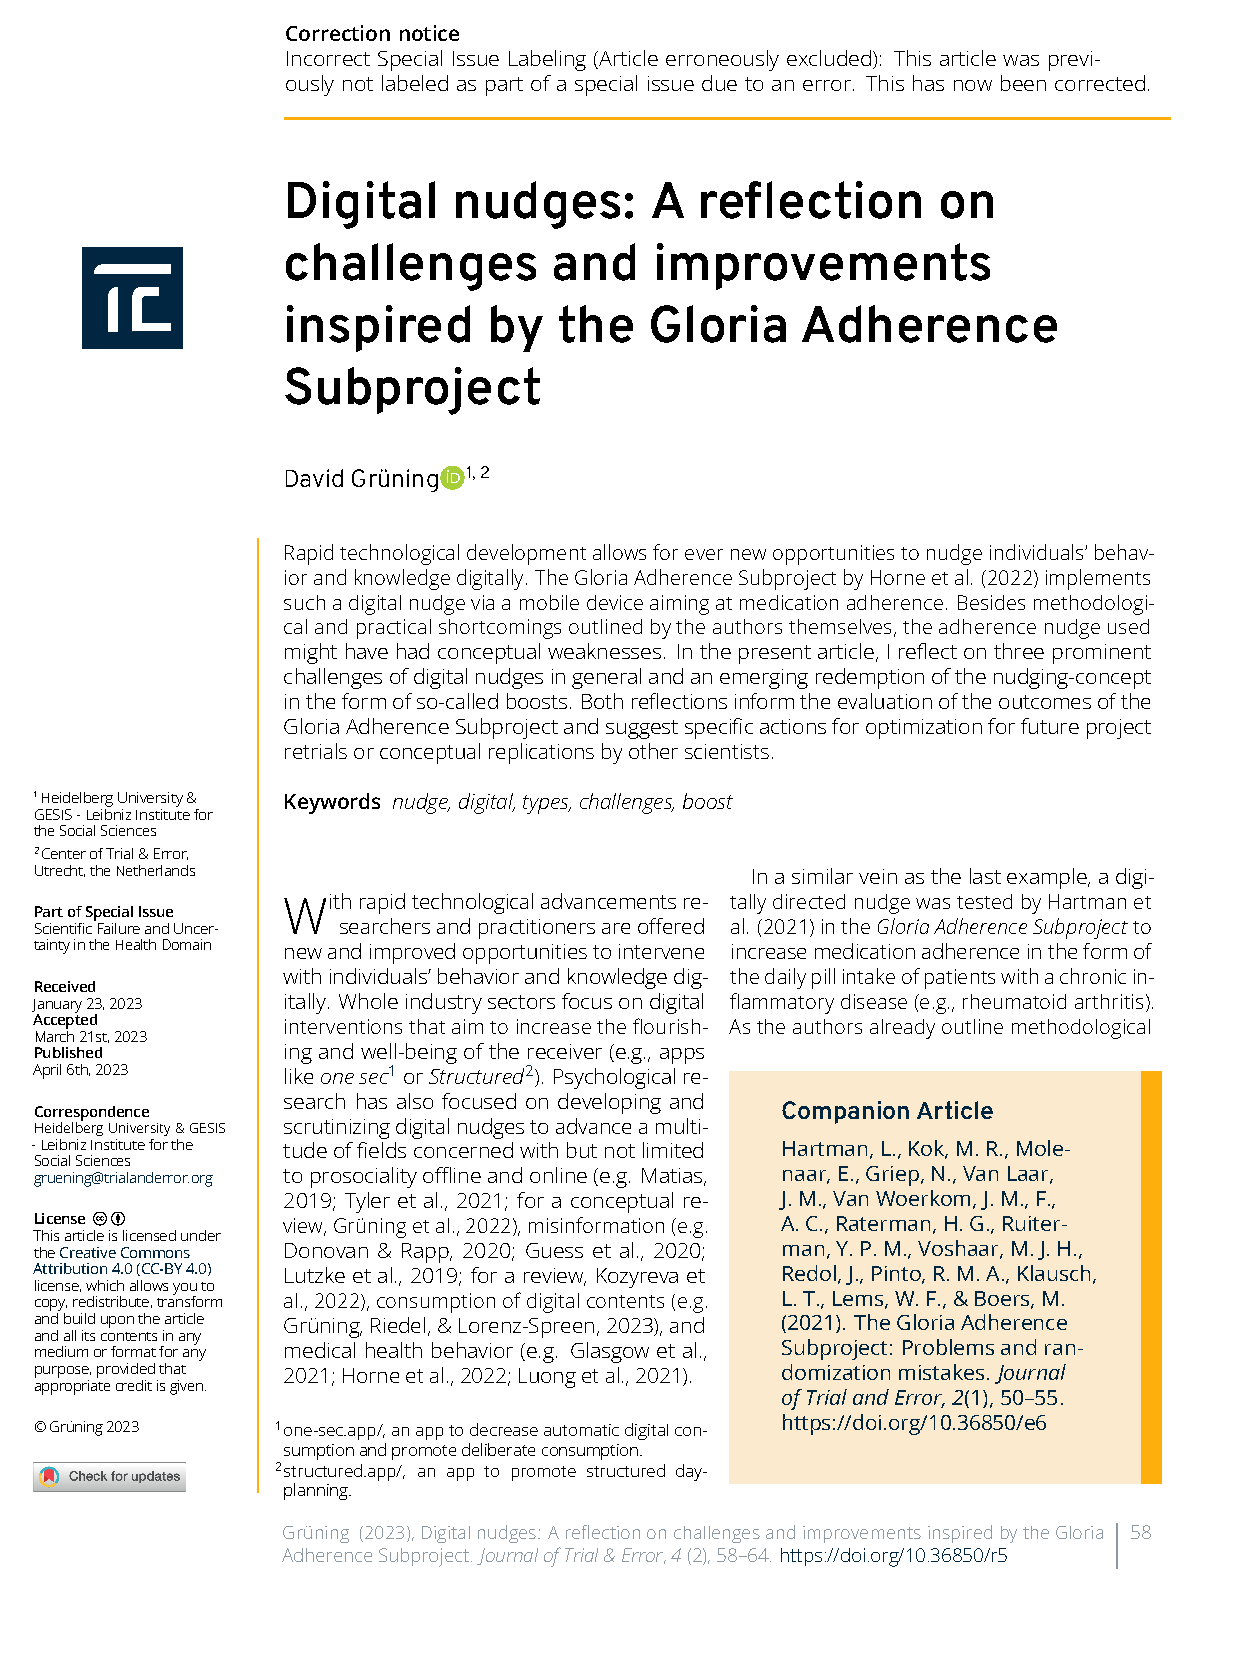
\includepdf[pages=-]{7 gruening nudges/gruening.pdf}

\includepdf[pages=-]{8 hromatko/main.pdf}

\includepdf[pages=-]{9 schleim reflections/main.pdf}

\includepdf[pages=-]{10 lind smile/main.pdf}

\includepdf[pages=-]{11 reitsema smile/main.pdf}

\includepdf[pages=-]{12 terstappen retrospective/main.pdf}

\includepdf[pages=-]{13 bakhuis era/main.pdf}

\includepdf[pages=-]{14 wisse pentacon/main.pdf}

\includepdf[pages=-]{15 wisse reflection/main.pdf}
% ... add a line for every PDF file you have

\end{document}